\chapter{Additional Plots}\label{Additional plots appendix}

\begin{figure}[ht]
    \centering
    \begin{subfigure}[b]{0.48\textwidth}
        \centering
        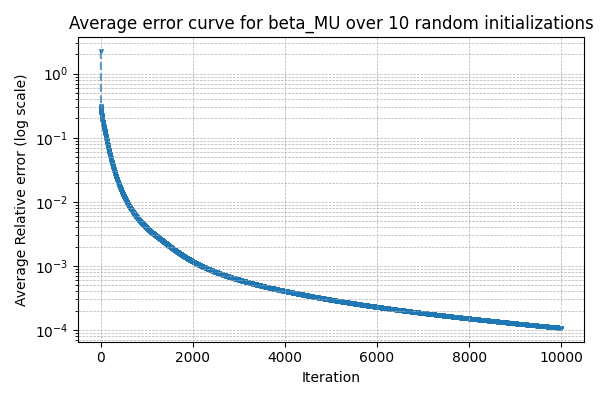
\includegraphics[width=\linewidth]{Imgs/Chapter 5/Appendix plots/MU_beta_0_average_random_10init.png}
        \caption{Reconstruction error vs. number of iterations for MU algorithm on synthetic data with $\beta=0$.}
        \label{fig:MU_beta_0}
    \end{subfigure}
    \hfill
    \begin{subfigure}[b]{0.48\textwidth}
        \centering
        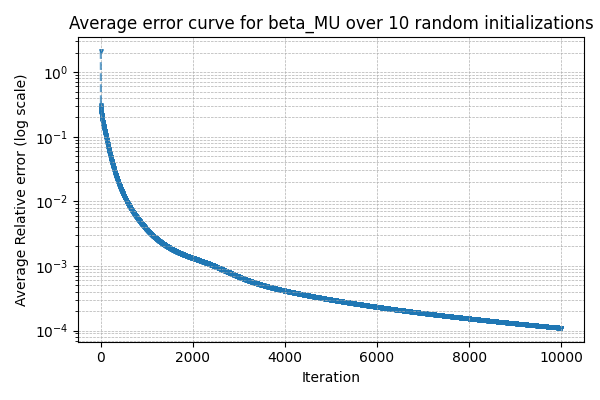
\includegraphics[width=\linewidth]{Imgs/Chapter 5/Appendix plots/MU_beta_1_average_random_10init.png}
        \caption{Reconstruction error vs. number of iterations for MU algorithm on synthetic data with $\beta=1$.}
        \label{fig:MU_beta_1}
    \end{subfigure}

    \vspace{0.5cm} % vertical space between rows 

    \begin{subfigure}[b]{0.48\textwidth}
        \centering
        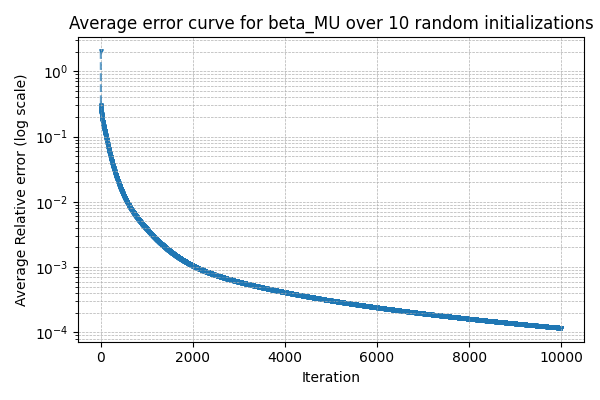
\includegraphics[width=\linewidth]{Imgs/Chapter 5/Appendix plots/MU_beta_2_average_random_10init.png}
        \caption{Reconstruction error vs. number of iterations for MU algorithm on synthetic data with $\beta=2$.}
        \label{fig:MU_beta_2}
    \end{subfigure}
    \hfill
    \begin{subfigure}[b]{0.48\textwidth}
        \centering
        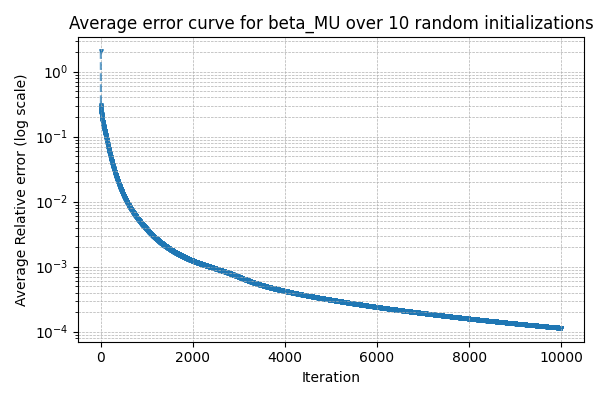
\includegraphics[width=\linewidth]{Imgs/Chapter 5/Appendix plots/MU_beta_3_2_average_random_10init.png}
        \caption{Reconstruction error vs. number of iterations for MU algorithm on synthetic data with $\beta=3/2$.}
        \label{fig:MU_beta_3_2}
    \end{subfigure}

    \caption{Reconstruction error versus number of iterations for the MU algorithm on synthetic data for various $\beta$ values.}
    \label{fig:MU_all_beta}
\end{figure}


\begin{figure}[ht]
    \centering
    \begin{subfigure}[b]{0.48\textwidth}
        \centering
        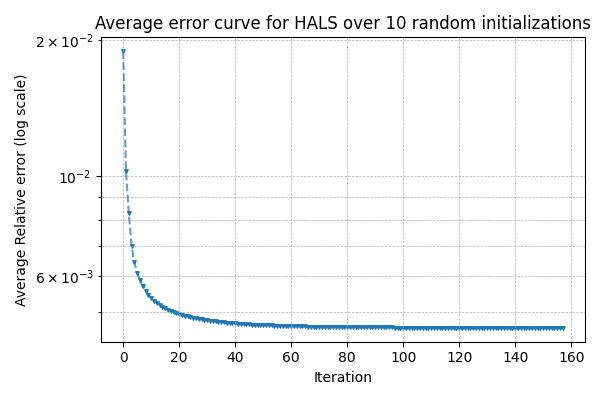
\includegraphics[width=\linewidth]{Imgs/Chapter 5/Appendix plots/HALS_average_random_10init.png}
        \caption{HALS}
        \label{fig:HALS_synthetic}
    \end{subfigure}
    \hfill
    \begin{subfigure}[b]{0.48\textwidth}
        \centering
        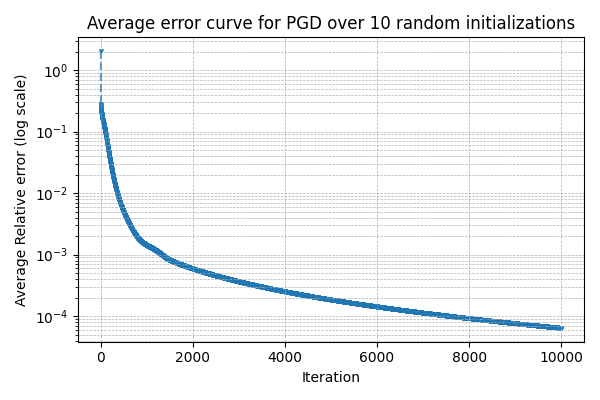
\includegraphics[width=\linewidth]{Imgs/Chapter 5/Appendix plots/PGD_average_random_10init.png}
        \caption{PGD}
        \label{fig:PGD_synthetic}
    \end{subfigure}
    \vspace{0.5cm}
    \begin{subfigure}[b]{0.48\textwidth}
        \centering
        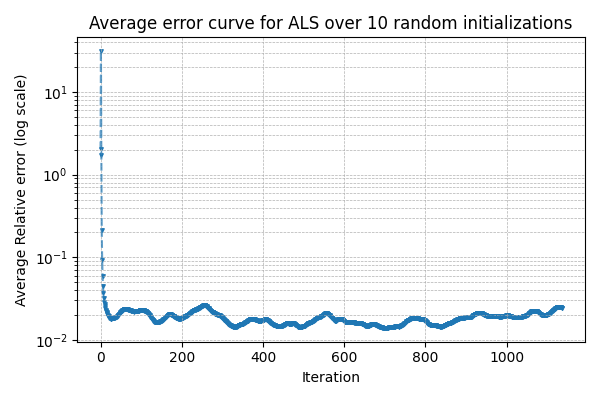
\includegraphics[width=\linewidth]{Imgs/Chapter 5/Appendix plots/ALS_average_random_10init.png}
        \caption{ALS}
        \label{fig:ALS_synthetic}
    \end{subfigure}
    \caption{Reconstruction error vs. number of iterations for HALS, PGD, and ALS algorithms on synthetic data.}
    \label{fig:HALS_PGD_ALS_synthetic}
\end{figure}


% \subsection{Olivetti Dataset}

\begin{figure}
    \centering
    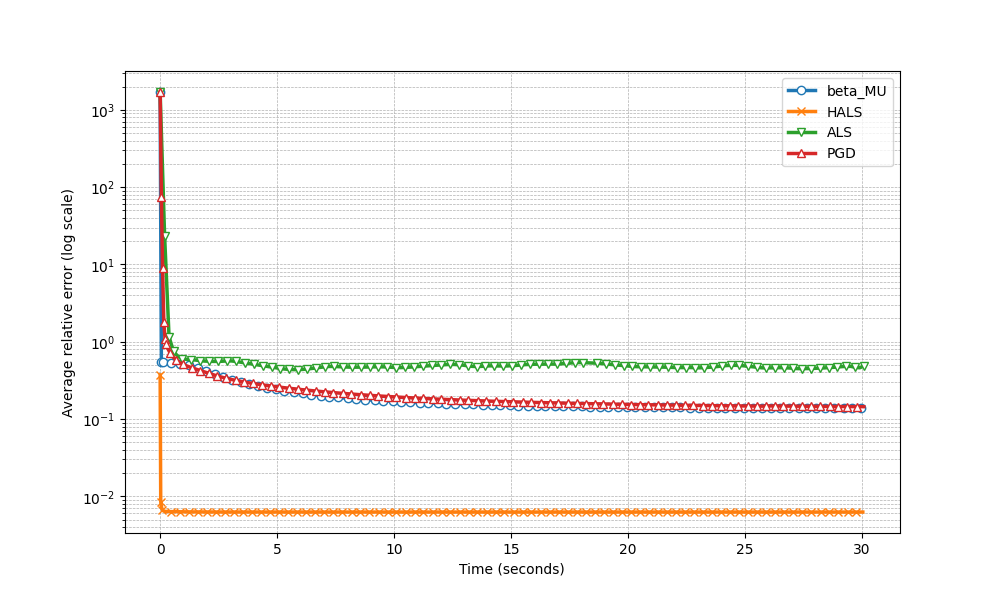
\includegraphics[width=1\textwidth]{Imgs/Chapter 5/Appendix plots/Olivetti_dataset_random_init.png}
    \caption{Average reconstruction error for different algorithms averaged over 10 random initializations on the Olivetti dataset.}
    \label{fig:Olivetti dataset}
\end{figure}


% low rank


\begin{figure}[ht]
    \centering
    \begin{subfigure}[b]{0.48\textwidth}
        \centering
        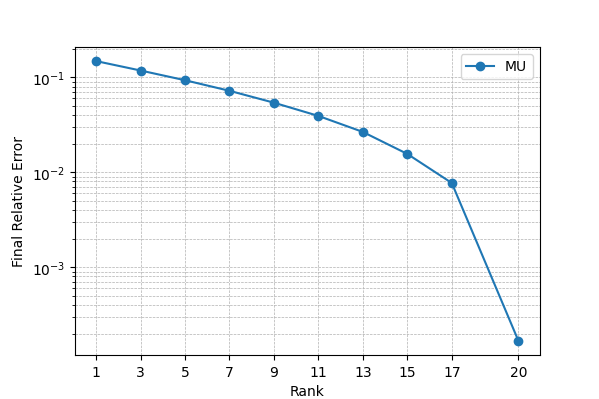
\includegraphics[width=\linewidth]{Imgs/Chapter 5/Rank_MU.png}
        \caption{Reconstruction error vs. rank for MU algorithm on synthetic data with $\beta = 2$.}
        \label{fig:MU_beta_2_rank}
    \end{subfigure}
    \hfill
    \begin{subfigure}[b]{0.48\textwidth}
        \centering
        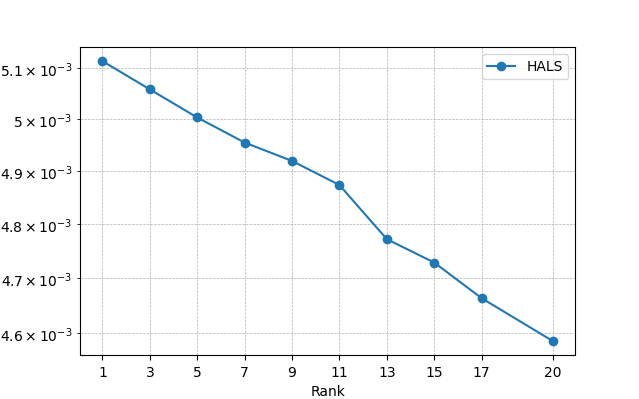
\includegraphics[width=\linewidth]{Imgs/Chapter 5/Rank_HALS.png}
        \caption{Reconstruction error vs. rank for HALS algorithm on synthetic data.}
        \label{fig:HALS_rank}
    \end{subfigure}

    \vspace{0.5cm} % vertical space between rows 

    \begin{subfigure}[b]{0.48\textwidth}
        \centering
        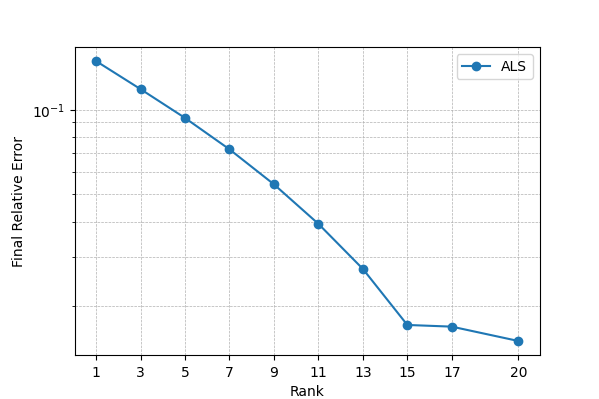
\includegraphics[width=\linewidth]{Imgs/Chapter 5/Rank_ALS.png}
        \caption{Reconstruction error vs. rank for ALS algorithm on synthetic data.}
        \label{fig:ALS_rank}
    \end{subfigure}
    \hfill
    \begin{subfigure}[b]{0.48\textwidth}
        \centering
        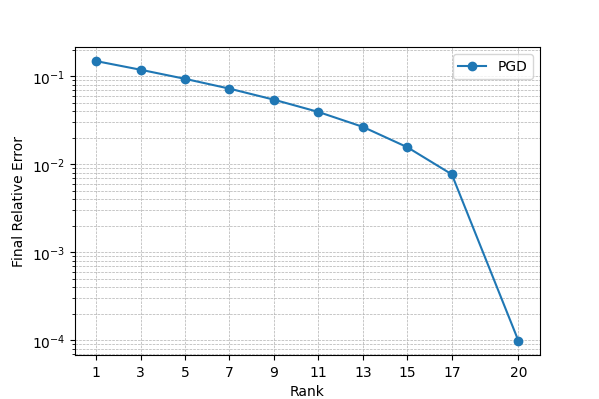
\includegraphics[width=\linewidth]{Imgs/Chapter 5/Rank_PGD.png}
        \caption{Reconstruction error vs. rank for PGD algorithm on synthetic data.}
        \label{fig:PGD_rank}
    \end{subfigure}

    \caption{Final reconstruction error versus reconstruction rank for different solvers.}
    \label{fig:error_vs_rank}
\end{figure}